\section{Evaluation}
\label{section:evaluation}

%
% power consumption of the ATTiny85
%
\begin{table*}%[h!]
  \begin{center}
  
  \begin{tabular}{| c | c | c |}

  \hline
  \textbf{Mode} & \textbf{Typical Consumption} & \textbf{Max Consumption} \\
  \hline
  Active      & 5 mA & 8 mA \\
  Idle        & 1.2 mA & 2 mA \\
  Power-Down  & 2 $\mu$A & 2 $\mu$A \\
  \hline
  
  \end{tabular}
  \end{center}
  \caption{Power Consumption of ATTiny85 Modes at 8 MHz at 3V.
  \label{table:attiny85_power}  
  }
\end{table*}

%
% power consumption of the CC2500
%
\begin{table*}%[h!]
  \begin{center}
  
  \begin{tabular}{| c | c | c |}

  \hline
  \textbf{Mode} & \textbf{Minimum Consumption} & \textbf{Max Consumption} \\
  \hline
  Power-Down        & 400 nA & 160 $\mu$A \\
  Idle              & 1.2 mA & 2 mA \\
  Temperature-Read  & 1.5 mA & 1.5 mA \\
  TX Mode (2.4 Kbaud) & 11.1 mA & 21.5 mA \\
  RX Mode (2.4 Kbaud) & 14.5 mA & 17.0 mA \\
  \hline
  
  \end{tabular}  
  \end{center}
  \caption{Power Consumption of the CC2500 modes at 3V.
  \label{table:cc2500_power}  
  }
\end{table*}

%
% bill of materials
%
\begin{table*}%[h!]
  \begin{center}
  
  \begin{tabular}{| c | c | c | c |}

  \hline
  \textbf{Equipment} & \textbf{Cost at 1} & \textbf{Cost at 10} & \textbf{Cost at 100} \\
  \hline
  ATTiny85-20PU     & \$1.29 & \$1.08 & \$0.74 \\
  CC2500            & \$1.29 & \$1.08 & \$0.74 \\
  Battery (CR2450)  & \$1.29 & \$1.08 & \$0.74 \\
  Total             & \$1.29 & \$1.08 & \$0.74 \\
  \hline
  
  \end{tabular}  
  \end{center}
  \caption{Bill of Materials and Per-Part Cost on Different Scales of Production (as of November 2013).
  \label{table:bill}
  }
\end{table*}

%
% power consumption
%
\begin{table*}
  \begin{center}
  
  \begin{tabular}{| c | c | c |}

  \hline
  \textbf{Mode} & \textbf{Calculated} & \textbf{Measured} \\
  \hline
  Power-Down        & 2.4 $\mu$A & \\
  Idle              & & \\
  Temp Read         & & \\
  TX Read           & & \\
  RX Read           & & \\
  \hline
  
  \end{tabular}  
  \end{center}
  \caption{Power consumption.
  \label{table:power_consumption}
  }
\end{table*}

In this section we describe our investigation into sensor node communication. We built the nodes in software 

\subsection{Software Simulation}

Software simulation of the nodes was performed using Contiki OS. 

\subsection{Hardware}

As the primary purpose of this project is to produce inexpensive sensor networks, we built 20 nodes over a 2-week period. The total cost was \$158.60. After our hardware arrived we proceeded to run two experiments: one investigating power consumption, and one investigating large network tests.

\subsubsection{Hardware Costs}

Table 3 shows the overall parts cost. CC2500 and ATTiny costs were taken from Mouser.com. CR2450 cost information came from Amazon for cost at 1, and AliExpress for cost at 10 and 1000. Costs not included are PCB fabrication, as the system has not left the breadboard phase at the time of this writing. Also not included are shipping costs as the lightweight nature of the components (The heaviest component being the battery at 6.8 grams) meant that shipping was not a significant cost at any magnitude. The breadboard prototypes cost a total of \$7.59 per unit.

\subsubsection{Power Consumption}

We ran int

\subsection{Intercommunication}

\begin{figure}[h!]
  \centering
  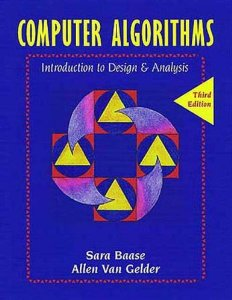
\includegraphics[width=0.5\textwidth]{images/textbook.png}
  \caption{Project cost measured in textbooks.
  \label{img:flowchart}
  }
\end{figure}

\begin{figure}[h!]
  \centering
  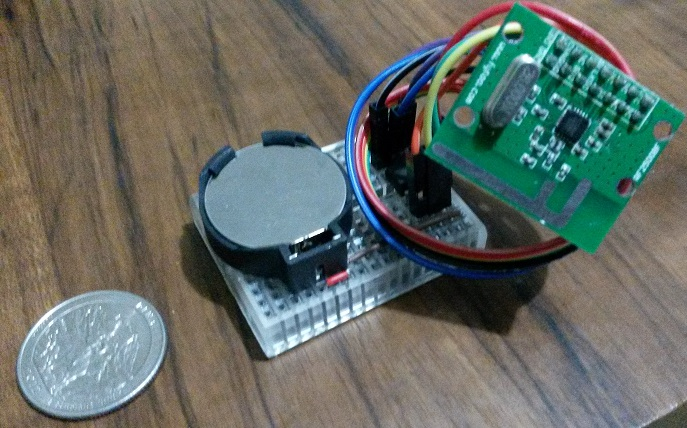
\includegraphics[width=0.5\textwidth]{images/phone_picture.png}
  \caption{Node on a breadboard.
  \label{img:flowchart}
  }
\end{figure}

While 20 nodes are fine for hardware simulation, we wanted to investigate a more realistic number of sensor nodes. However, it is not possible to install ContikiOS onto the microcontroller due to memory limitations. To enable communication in between the hardware and the software simulation we added an ATMega128RFA1. This microcontroller has a built-in Zigbee-compatible transceiver and is capable of running ContikiOS natively.
